\documentclass{article}
\usepackage[utf8]{inputenc}
\usepackage{indentfirst}
\usepackage{amsmath}
\usepackage{amsthm}
\usepackage{graphicx}
\usepackage{float}
\title{RL Crash Course + Some Thoughts}
\author{Ding (Eric) Ding}
\date{November 2022}
\begin{document}

\maketitle

\section{Introduction}
    In this Project, I followed OpenAI deep reinforcement learning course, and used Spinning Up for exercises and experiments.

\section{What's Omitted}
    Regularization, Observation normalization

\section{Key Concepts}
    The main characters of RL are the agent and the environment. The environment is the world that the agent lives in and interacts with. At every step of interaction, the agent sees a (possibly partial) observation of the state of the world, and then decides on an action to take. The environment changes when the agent acts on it, but may also change on its own.
    \begin{figure}[H]
        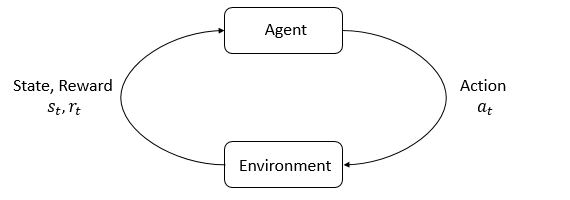
\includegraphics[width=\linewidth]{rl_diagram_transparent_bg.png}
        \caption{RL framework}
        \label{fig:rl}
      \end{figure}

    The agent also perceives a reward signal from the environment, a number that tells it how good or bad the current world state is. The goal of the agent is to maximize its cumulative reward, called return. Reinforcement learning methods are ways that the agent can learn behaviors to achieve its goal.

    States and observations: represented by matrix

    Action Spaces: the set of all valid actions. Discrete / continuous.

    Policies: a rule used by an agent to decide what actions to take. Deterministic: $a_t = \mu_{\theta}(s_t)$. Stochastic: $a_t \sim \pi_{\theta}(\cdot | s_t)$. In deep RL, we deal with parametrized policies, with parameters that can be adjusted by optimization. 
    
    Stochastic policies: categorical policies in discrete action space and diagonal gaussian policies in continuous action spaces. Two key computations: sampling actions from the policy, and compute log likelihoods of particular actions.

    Trajectory: A sequence of states and actions in the world. Can be deterministic or stochastic based on policy. 

    Reward and return: $r_t = R(s_t, a_t, s_{t+1})$. Maximize cumulative return $R(\tau)$. Finite-horizon undiscounted return: $R(\tau) = \Sigma_{t = 0} ^T r_t$. Infinite-horizon discounted return: $R(\tau) = \Sigma_{t =0} ^{\infty}\gamma^tr_t$

    The goal in RL is to select a policy which maximizes expected return when the agent acts according to it. The probability of a trajectory: 
    $$P(\tau | \pi) = \rho_0(s_0) \prod_{t = 0} ^{T - 1} \pi(a_t | s_t) P(s_{t+1}|s_t, a_t)$$
    The expected return is:
    $$
    J(\pi) = \int_\tau P(\tau | \pi) R(\tau) = E_{\tau \sim \pi} [R(\tau)]
    $$
    The central optimization problem in RL can then be expressed by
    $$
    \pi^* = \arg\max_\pi J(\pi)
    $$

    Value functions: it's useful to know the value of a state, which is the expected return if start in that state. 1) On-Policy Value Function $V^\pi(s)$, start in state $s$ and always acts according to policy $\pi$. 2) On-Policy Action-Value Function $Q^\pi(s, a)$, start in state $s$, take arbitrary action $a$, and then acts according to policy $\pi$. 3) Optimal Value Function $V^*(s)$, start in state $s$ and acts according to the optimal policy. 4) Optimal Action Value Function $Q^*(s, a)$. 

    The Optimal Q-Function and the Optimal Action: $a^*(s) = \arg\max_a Q^*(s, a)$

    Bellman Equations: 
    $$
      V^\pi(s) = E_{a \sim \pi, s' \sim P}[r(s,a) + \gamma V^\pi(s')]
    $$
    $$
      Q^\pi(s, a) = E_{s' \sim P} [r(s, a) + \gamma E_{a' \sim \pi}[Q^\pi(s', a')]]
    $$
    $$
      V^*(s ) = \max_a E_{s' \sim P} [r(s, a) + \gamma V^*(s')]
    $$
    $$
      Q^*(s, a) = E_{s' \sim P} [r(s, a) + \gamma \max_{a'} Q^*(s', a')]
    $$

    Advantage Function:
      $$
        A^\pi(s, a) = Q^\pi(s, a) - V^\pi(s)
      $$

\section{Kinds of RL Algorithm}
  \begin{figure}[H]
    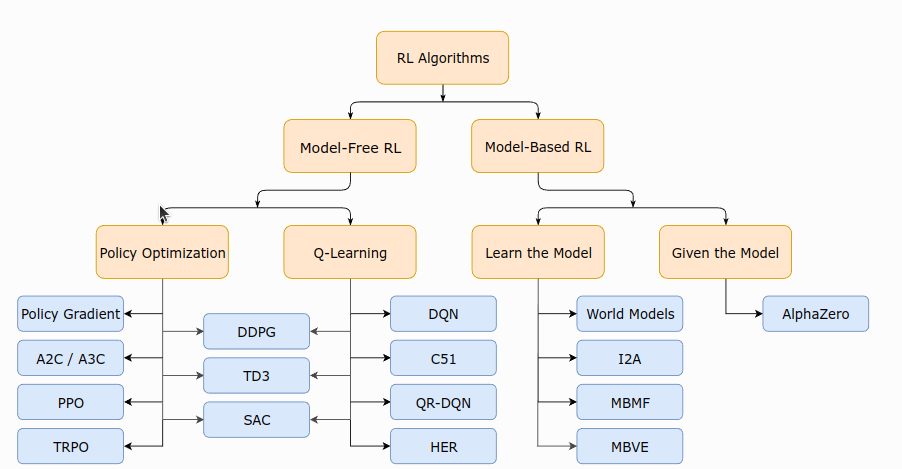
\includegraphics[width=\linewidth]{rlalg.png}
    \caption{RL Algorithm}
    \label{fig:ag}
  \end{figure}
  \subsection{Model-Free vs. Model-Based}
    Whether the agent has access to (or learns) a model of the environment. The model is a function that predicts state transitions and rewards.

    Model allows the agent to think ahead. Such a model is usually not available to the agent. If there is no such models, it has to learn the model purely from experience.  The biggest challenge is that bias in the model can be exploited by the agent, resulting in an agent which performs well with respect to the learned model, but behaves sub-optimally (or super terribly) in the real environment.

    While model-free methods forego the potential gains in sample efficiency from using a model, they tend to be easier to implement and tune. 
  \subsection{What to Learn}
    \begin{enumerate}
      \item Policies
      \item Action-value functions
      \item Value functions
      \item Environment models
    \end{enumerate}
  \subsection{What to Learn in Model-Free RL}
    \begin{enumerate}
      \item Policy Optimization: $\pi_\theta(a|s)$. It optimizes the parameters $\theta$ either directly by gradient ascent on the performance objective $J(\pi_{\theta})$, or indirectly, by maximizing local approximations of $J(\pi_{\theta})$. This is always performed on-policy, each update only uses data collected while acting according to the most recent version of the policy. Also involves learning an approximator $V_\phi(s)$ for the on-policy value function $V^\pi(s)$
      \item Q-Learning: Learn an approximator $Q_\theta(s, a)$ for the optimal action-value function $Q^*(s, a)$. This optimization is almost always performed off-policy, each update can use data collected at any point during training. $a(s) = \arg\max_a Q_\theta(s, a)$
    \end{enumerate}

    Policy Optimization is more stable and reliable, but less sample efficient.
  \subsection{What to Learn in Model-Based RL}
    \begin{enumerate}
      \item Background: Pure Planning. Each iteration, the agent observes the model, computes a plan with respect to the model (use learned value function)
      \item Expert iteration:  Using and learning an explicit representation of the policy. Uses a planning algorithm to generate candidate actions for the plan by sampling from the current policy.
      \item Data augmentation for Model-Free methods
      \item Embedding planning loops into policies
    \end{enumerate}
\section{Policy Optimization}
    Want to maximize the expected return $J(\pi_{\theta}) = E_{\tau \sim \pi_{\theta}}[R(\tau)]$. $R(\tau)$ gives the finite-horizon undiscounted return.
    
    We would like to optimize the policy by gradient ascent, 
    $$
    \theta_{k+1} = \theta_k + \alpha \nabla_{\theta} J(\pi_{\theta})|_{\theta_k}.
    $$

    How to numerically compute the policy gradient? This involves two steps: 1) deriving the analytical gradient of policy performance, which turns out to have the form of an expected value, and then 2) forming a sample estimate of that expected value, which can be computed with data from a finite number of agent-environment interaction steps.
    \begin{figure}[H]
      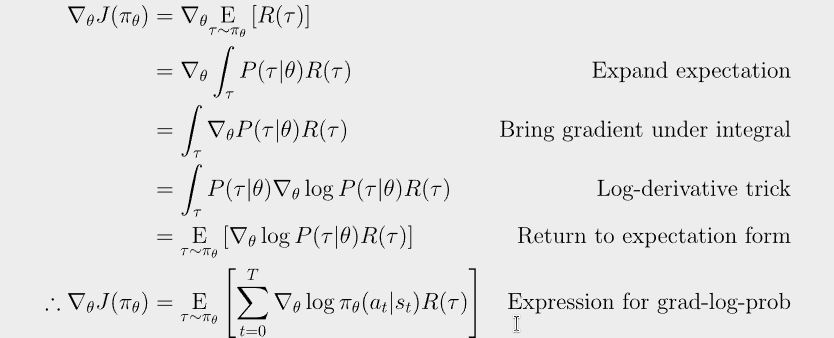
\includegraphics[width=\linewidth]{derivative.png}
      \caption{Policy Gradient}
      \label{fig:policygradient}
    \end{figure}

    The policy gradient can be estimated with: 
    $$
    \hat{g} = \frac{1}{|\mathcal{D}|} \sum_{\tau \in \mathcal{D}} \sum_{t=0}^{T} \nabla_{\theta} \log \pi_{\theta}(a_t |s_t) R(\tau),
    $$
    $\mathcal{D} = \{\tau_i\}_{i=1,...,N}$ is the set of trajectories.


\section{Ideas}
    \subsection{Observation}
      Fully observed environment vs. partially observed\
    \subsection{Action}
      Rule out certain actions in action space, can combine both stochastic and deterministic policy.
    \subsection{Value}\
      How to calculate value functions (future) and adjust policy accordingly (optimize)? 

\end{document}